% =============================================================================
% Revised Methodology section for the HERMES / FeRRy paper.
%
% HOW TO USE
%   This file compiles on its own (IEEEtran, conference). To merge it into
%   Hermes_paper.tex, copy everything between the two markers
%       %%%%% BEGIN SECTION %%%%%   and   %%%%% END SECTION %%%%%
%   and replace the old text from "\section{HERMES Methodology}" through the end
%   of "Layer 3" (including both algorithms and the old complexity paragraph).
%   Then add the \newcommand lines and the packages listed in the preamble below
%   to your own preamble.
%
%   \sysname is one switch for the system name. The arms tables and figures call
%   the system FeRRy; if the paper keeps HERMES, change \sysname here and
%   regenerate the tables and figures with the new label.
%
% NEW BIB KEYS THIS SECTION CITES (add to biblio.bib; the rest already exist)
%   xie2019asynchronous  FedAsync (hinge staleness form)
%   zeng2019energy       Zeng, Xu, Zhang, rotary-wing UAV energy model, 2019
%   3gpp36104            3GPP TS 36.104, channel bandwidth / N_RB table
%   3gpp36777            3GPP TR 36.777, UAV channel model parameters
%   (CICIoT2023 is cited as CiCIoT2023, already in biblio.bib)
%
% Every number below was checked against the code at commit 9a02a68 (7 Oct 2026;
% hermes/ and experiments/ are unchanged through 11671f7). Corrections applied on
% 8 Oct 2026: the mission budget bounds Pass 1 only; occupied bandwidth; the
% interference term, its phases and sigma_I; the hashing keys; the S* rule; the
% evaluated feasibility clauses; the empty-mask fallback; the search modes; the
% backhaul in the evaluated configuration; merge ages; Pass 2's conditions; the
% names F and FX. Added: the learning task, contact outcomes, several mules,
% device training time, and FerrySim. Radio quantities are simulated; none is an
% AERPAW measurement.
% =============================================================================
\documentclass[conference]{IEEEtran}
\IEEEoverridecommandlockouts

\usepackage[utf8]{inputenc}
\usepackage{cite}
\usepackage{amsmath,amssymb,amsfonts}
\usepackage{graphicx}
\usepackage{booktabs}
\usepackage{tabularx}
\usepackage{array}
\usepackage[table]{xcolor}
\usepackage{algorithm}
\usepackage{algpseudocode}
\usepackage{tikz}
\usetikzlibrary{positioning, arrows.meta, calc}

\newcolumntype{L}{>{\raggedright\arraybackslash}X}
\newcommand{\sysname}{FeRRy}
\newcommand{\bbar}{\bar{b}}
\newcommand{\Tnom}{T_{\mathrm{nom}}}

\begin{document}
\title{Revised Methodology Section (drop-in)}
\maketitle

%%%%% BEGIN SECTION %%%%%
\section{\sysname{} Methodology}
\label{sec:method}

\sysname{} sustains federated learning across regions that a stationary network
cannot reach, by sending an autonomous mule (UAV) between edge devices and an
edge server. This section describes what the mule decides, when it decides it,
and which quantities each decision uses. We organize the description by
\emph{decision clock} rather than by layer, because the two decisions that
determine most of the behavior of the system each span the radio, scheduling,
and learning layers. Section~\ref{sec:method:roles} fixes the setting and the
role of each layer, Section~\ref{sec:method:models} defines the quantities that
the layers supply, Sections~\ref{sec:method:gate}--\ref{sec:method:flight}
define the shared feasibility test and the two decision clocks, and
Section~\ref{sec:method:merge} defines aggregation. Section~\ref{sec:method:alg}
gives the complete mission round, its cost, and the implementation.

% -----------------------------------------------------------------------------
\subsection{Setting, Layer Roles, and Decision Clocks}
\label{sec:method:roles}

\paragraph{Setting}
A cluster consists of one edge server, one or more mules, and a set of field
devices. The server holds the device registry and assigns each mule a disjoint
slice $\mathcal{M}$ of it. Devices train their local model offline between
visits, so a contact is exchange only: the mule pushes the current global model
and pulls the device's prepared update. A \emph{mission} has two passes. In
\textsc{Pass 1} the mule collects updates along a route, merges them on board,
and docks to upload the merged result. The server merges across mules and
produces the next global model. In \textsc{Pass 2} the mule delivers that model
to every device in its slice. Delivering a known model version in Pass~2 is what
gives each collected update an observable basis version, and therefore an age
(Section~\ref{sec:method:models}). Each mission has a time budget
$T_{\mathrm{miss}}$ that bounds Pass~1: the mule must land and finish its upload
within $T_{\mathrm{miss}}$ of takeoff. Pass~2 is not budgeted.

\paragraph{Several mules}
With $K>1$ mules, the server cuts the field into $K$ contiguous sectors by angle
around the dock, starting after the widest empty arc, with slice sizes that
differ by at most one device. Every mule starts at the shared dock, and the mules
fly concurrently. Each mule plans and flies its own slice, and the server folds
the uploads in simulated-time order (Section~\ref{sec:method:merge}). Queueing at
the dock is not modelled.

\paragraph{Learning task}
The devices train a binary intrusion detector on CICIoT2023~\cite{CiCIoT2023}.
Every flow is labelled benign or attack (the 33 attack labels form one class) and
is described by 21 features scaled to $[0,1]$. Each trial draws 20{,}000
training flows, half of them benign, and a disjoint test set of 6{,}000 flows,
4{,}000 of them benign. The training flows are split evenly at random across the
$N$ devices, about 3{,}333 per device at $N=6$. The model is a multilayer
perceptron with hidden layers of 64, 32, 16, 8 and 4 units (ReLU, batch
normalization, dropout 0.4, $L_2$ weight $10^{-3}$) and a sigmoid output, trained
with Adam (learning rate $10^{-3}$) on binary cross-entropy. A device trains one
local epoch (batch 64) per model it receives: offline after each Pass-2 delivery,
or at its first Pass-1 contact, before any delivery has reached it. After each
round closes, the server evaluates the global model on the test set; the
accuracy at a 0.5 threshold is the quantity the target $\tau$ refers to
(Section~\ref{sec:setup:cells}). The model occupies 18.8~KB; to represent a
larger model, every transfer is priced as if it held $S=1$~MB
(Section~\ref{sec:method:l1}).

\paragraph{What the layers contribute}
Table~\ref{tab:layer-roles} states the role of each layer in the decisions
below. The radio layer prices a link; it does not choose among devices. The
scheduling layer makes every route and band decision. The learning layer
supplies the value of a collected update and the cost of an uncollected one.
Hard gates (eligibility, the feasibility test of
Section~\ref{sec:method:gate}, and the age cap) always run before any ranking
step, so a ranking rule, learned or not, only chooses among options that the
gates have admitted.

\begin{table}[t]
\centering
\caption{Role of each layer in the joint decisions.}
\label{tab:layer-roles}
\small
\begin{tabularx}{\columnwidth}{l l L}
\toprule
\textbf{Layer} & \textbf{Role} & \textbf{Supplies to the decisions} \\
\midrule
L1 RF link & prices & Range, rate, dwell, and SNR over time for each band class; backhaul carrier \\
L2 Scheduling & decides & Admission, band class $\bbar$, route, per-arrival (band, next stop), re-plan \\
L3 Federated learning & values & Merge weight, update age, coverage weight, cross-mule merge \\
\bottomrule
\end{tabularx}
\end{table}

\paragraph{Two decision clocks}
The mule decides on two clocks, shown in Fig.~\ref{fig:clocks}. On the
\emph{plan clock}, once per mission at the dock, it chooses a contact band class
$\bbar$ and an ordered route together, because the band class fixes the contact
range, the range fixes how devices cluster into stops, and the stops fix the
route. On the \emph{flight clock}, at every Pass-1 arrival, it chooses the band
for the current stop and the next stop together, using the signal it observes at
that moment. The separation matters because the channel varies within a single
sortie: interference has a period comparable to the duration of a leg, so the
band that is best at takeoff need not be best at a later stop. A third element,
the \emph{return path}, carries what the flight observes back to the plan. Rate
sets dwell, dwell advances the mission clock, the clock decides feasibility, and
infeasibility triggers a re-plan.

\begin{figure}[t]
\centering
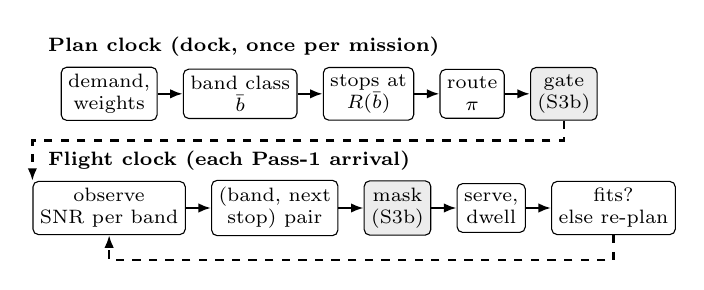
\begin{tikzpicture}[
  box/.style={draw, rounded corners=2pt, minimum height=0.62cm, align=center,
              font=\scriptsize, inner sep=2.5pt},
  gate/.style={box, fill=gray!15},
  arr/.style={-{Latex[length=1.6mm]}, thick},
  node distance=0.32cm]
  % plan clock
  \node[font=\scriptsize\bfseries, anchor=west] (pl) at (0,1.55) {Plan clock (dock, once per mission)};
  \node[box] (d) at (0.9,0.95) {demand,\\weights};
  \node[box, right=of d] (bb) {band class\\$\bbar$};
  \node[box, right=of bb] (st) {stops at\\$R(\bbar)$};
  \node[box, right=of st] (rt) {route\\$\pi$};
  \node[gate, right=of rt] (g1) {gate\\(S3b)};
  \draw[arr] (d)--(bb); \draw[arr] (bb)--(st); \draw[arr] (st)--(rt); \draw[arr] (rt)--(g1);
  % flight clock
  \node[font=\scriptsize\bfseries, anchor=west] (fl) at (0,0.1) {Flight clock (each Pass-1 arrival)};
  \node[box] (ob) at (0.9,-0.5) {observe\\SNR per band};
  \node[box, right=of ob] (pr) {(band, next\\stop) pair};
  \node[gate, right=of pr] (g2) {mask\\(S3b)};
  \node[box, right=of g2] (sv) {serve,\\dwell};
  \node[box, right=of sv] (rp) {fits?\\else re-plan};
  \draw[arr] (ob)--(pr); \draw[arr] (pr)--(g2); \draw[arr] (g2)--(sv); \draw[arr] (sv)--(rp);
  \draw[arr, dashed] (rp.south) -- ++(0,-0.32) -| (ob.south);
  \draw[arr, dashed] (g1.south) -- ++(0,-0.25) -| (ob.north west);
\end{tikzpicture}
\caption{The two decision clocks. The shaded boxes are the same feasibility test,
applied once to the committed plan and again to every candidate pair in flight.}
\label{fig:clocks}
\end{figure}

\paragraph{What is learned}
Every decision on both clocks is made by a rule or a search over a declared
score. Learning can enter in one place only: a learned pair score can occupy the
flight slot in place of the fixed rule (Section~\ref{sec:method:flight}). We
therefore describe the design as a set of coupled decisions, and treat learning
as one optional way to fill one of them.

% -----------------------------------------------------------------------------
\subsection{Quantities Supplied by the Layers}
\label{sec:method:models}

\subsubsection{L1: Contact Link, Clock, and Backhaul}
\label{sec:method:l1}

\paragraph{Band classes}
The contact link offers a set $\mathcal{B}$ of band classes that differ in
occupied bandwidth, not in carrier. The three candidate carriers in our testbed
differ by at most 1.4~dB of free-space loss, which is too small to support a
range trade, so all classes share one carrier. We use three LTE channel
bandwidths~\cite{3gpp36104}: \textsf{wide} (20~MHz, 100 resource blocks),
\textsf{medium} (5~MHz, 25), and \textsf{narrow} (1.4~MHz, 6). Every rate and
range below uses the \emph{occupied} bandwidth $B_b=N_{\mathrm{RB}}\times
180$~kHz (18, 4.5 and 1.08~MHz). With a common transmit power and a noise floor
that scales with $B_b$, a narrower class reaches farther at a lower rate.
Relative to a reference class with bandwidth $B_0$ and slant range $R_0^{3D}$,
\begin{equation}
R_b^{3D} = R_0^{3D}\left(\frac{B_0}{B_b}\right)^{1/n},
\qquad
R_b = \sqrt{\left(R_b^{3D}\right)^2 - h^2},
\label{eq:range}
\end{equation}
where $n$ is the path-loss exponent and $h$ the UAV altitude. We anchor the
\textsf{wide} class at a planar range of 60~m with $h=25$~m and $n=2.2$, which
gives planar ranges of 60, 120 and 232~m for the three classes. This range is an
edge-availability range: at distance $R_b$ the mean SNR exceeds the decoding
floor by $M_{\mathrm{sh}}=\Phi^{-1}(0.9)\,\sigma_{\mathrm{sh}}=5.1$~dB, so a
device at the edge of its class is reachable with probability 0.9 under
shadowing alone (about 0.82 once the interference below is added).

\paragraph{Rate and dwell}
The mean SNR at distance $d$ under class $b$ is
\begin{equation}
\bar\gamma_b(d) = \gamma_{\mathrm{floor}} + M_{\mathrm{sh}}
  + 10\,n\log_{10}\!\frac{R_b^{3D}}{d^{3D}},
\label{eq:meansnr}
\end{equation}
with $\gamma_{\mathrm{floor}}=-6.7$~dB (CQI~1). The achievable rate is the
smaller of a CQI-table spectral efficiency and the Shannon rate on the occupied
bandwidth, and is zero below the floor:
\begin{equation}
r_b(\gamma)=\begin{cases}
\min\bigl\{\kappa_b B_b\,\mathrm{SE}(\gamma),\\
\quad B_b\log_2(1+10^{\gamma/10})\bigr\}, & \gamma\ge\gamma_{\mathrm{floor}},\\
0, & \text{otherwise,}
\end{cases}
\label{eq:rate}
\end{equation}
where $\kappa_b$ is an implementation efficiency factor and $\mathrm{SE}(\cdot)$
the CQI efficiency table. Transferring $S_j$ bytes to or from device $j$
therefore takes
\begin{equation}
\tau_{j,b}^{\mathrm{dwell}}(\gamma)=\frac{8S_j}{r_b(\gamma)}.
\label{eq:dwell}
\end{equation}
A Pass-1 session pushes the global model and pulls the update, so it is priced at
$S_j=2S$; a Pass-2 delivery and the upload at the dock are each priced at $S$.
The dwell times of the devices served at one stop add, because they share one
channel. A device whose SNR is below the floor at arrival is not solicited and
costs no airtime.

\paragraph{Channel over time}
The realized SNR of device $j$ on class $b$ at mission time $t$ is
\begin{equation}
\gamma_{b,j}(t)=\bar\gamma_b(d_j)+X_j(t)+I_b(t),
\label{eq:realsnr}
\end{equation}
where $X_j(t)$ is correlated shadowing ($\sigma_{\mathrm{sh}}=4$~dB, correlation
time 7.4~s) and
\begin{equation}
I_b(t)=A\sin\bigl(2\pi(t/P_c+\phi_b)\bigr)+\sigma_I\,\xi_b(t)
\label{eq:interf}
\end{equation}
is a per-class interference term~\cite{3gpp36777}: a periodic swing with period
$P_c=60$~s and a class-specific phase $\phi_b\in\{0,\tfrac13,\tfrac23\}$ of a
period, plus noise $\xi_b(t)$. In the interference-limited (``jittery'') regime
used throughout the evaluation, $A=5$~dB and $\sigma_I=1.5$~dB. Both terms are
generated from keyed hashes, so two policies that ask for the same value at the
same time receive the same value: shadowing is keyed by (seed, device, time) and
shared across classes, and the interference noise by (seed, class, time) and
shared across devices. The planner prices only the mean $\bar\gamma_b$. Pricing
the realized phase at plan time would be an oracle, so realized missions run
longer than planned, by an amount that grows as the class narrows. The flight
clock observes $\gamma_{b,j}(t)$. The planner also uses the probability that a
served device falls below the floor,
\begin{equation}
p_{\mathrm{out}}(b,d)=\Phi\!\left(\frac{\gamma_{\mathrm{floor}}-\bar\gamma_b(d)}{\sigma_{\mathrm{eff}}}\right),
\quad
\sigma_{\mathrm{eff}}^2=\sigma_{\mathrm{sh}}^2+\sigma_I^2+\tfrac{A^2}{2},
\label{eq:pout}
\end{equation}
a moment-matched approximation of the shadowing-plus-interference outage.

\paragraph{Mission clock and energy}
Mission time is a simulated clock charged with the physics of each step:
transit at cruise speed (5~m/s), dwell from Eq.~\eqref{eq:dwell}, a listen
window when an expected reply is missing, the return leg, the upload, and a
fixed dock turnaround of 30~s. Energy is a function of the same ledger,
\begin{equation}
E = P_{\mathrm{move}}\,(t_{\mathrm{transit}}+t_{\mathrm{return}})
  + P_{\mathrm{hover}}\,(t_{\mathrm{dwell}}+t_{\mathrm{listen}}),
\label{eq:energy}
\end{equation}
with $P_{\mathrm{move}}=143.6$~W and $P_{\mathrm{hover}}=168.5$~W from the
rotary-wing model of Zeng et al.~\cite{zeng2019energy}. This energy is
simulated, not measured, and no battery capacity is enforced in the evaluated
configuration.

\paragraph{Backhaul carrier}
The upload from mule to server rides one backhaul carrier. In the evaluated
configuration the mule holds the carrier with the largest effective-SNR gain
$g(c)$; the upload is timed at that carrier's mean SNR, and an upload is lost
with a fixed probability (2\% in the jittery regime), which decides whether a
cluster round closes. The radio layer also offers an adaptive controller that
re-scores the carriers before each upload by $U(c,t)=R\bigl(\gamma_1(t)+g(c)\bigr)
-\kappa(c)-\lambda(c,t)$, with $R(\cdot)$ an SNR-to-rate-tier map, $\kappa(c)$ a
use cost, and $\lambda(c,t)$ a switching cost. It is evaluated only as a
separate configuration (F+L1, Section~\ref{sec:setup:design}). The backhaul never
enters a scheduling decision.

\subsubsection{L2/L3: Demand, Deadlines, Ages, and the Age Cap}
\label{sec:method:demand}

\paragraph{Contact outcomes}
Each device served in Pass~1 ends its contact in one of three outcomes. It is
\emph{clean} when the device returns an update that matches the round, size and
checksum the mule expects, and \emph{partial} when it answers but refuses the
session or returns an update that fails those checks. Every other contact is a
\emph{timeout}: the device lies beyond the band's reach or below the decoding
floor at arrival, stays silent, fails the push, sends no reply, or has no update
ready. Whether a reachable device replies is drawn each mission from its
reliability $\rho_j$, drawn once per device and trial from $U(0.15,1)$. A missing
reply costs a 1~s listen window on the simulated clock. A session also has a
wall-clock timeout (36~s at $N=6$, set by a pilot as twice the 95th-percentile
fit time) that bounds how long the mule's process waits.

\paragraph{Device training time}
By default local training costs no simulated time, so an update is always ready
when the mule arrives. To study compute heterogeneity
(Section~\ref{sec:res:robust}), a device can instead take
$T_j=\tilde{T}\,e^{\sigma z_j}$ to train, with median $\tilde{T}$, $\sigma=0.5$,
and $z_j$ a keyed standard normal draw; a fixed share of the devices can be made
stragglers whose time is multiplied by a factor. A device's first fit starts at
the mule's first takeoff, and each model it receives restarts the fit. A device
whose update is not ready when the mule arrives answers but has nothing to send:
the contact is a timeout that costs no airtime and widens the device's window by
$\beta_{\mathrm{partial}}$ (Eq.~\eqref{eq:phi}). The plan does not price
training time.

\paragraph{Per-device deadline}
Each device $j$ carries a fulfilment window $\Phi(j)$ and a deadline
\begin{equation}
\mathrm{Deadline}(j)=t+\Phi(j)-\iota(j),
\label{eq:deadline}
\end{equation}
where $t$ is the planning time and $\iota(j)$ the time since the device's last
clean contact. The window starts at $\Phi_0=60\,\mathrm{s}\times\sigma$, where
the time scale $\sigma=\Tnom/10\,\mathrm{s}$ converts the unit in which the law
was first set to the duration of a simulated mission. $\Tnom$ is the median,
over 20 reference layouts of the cell, of the duration of one nominal two-pass
mission on the wide band with no budget and no failures (203~s at $N=6$ with one
mule). After each contact the window is multiplied by a factor that depends on
the outcome and clamped,
\begin{equation}
\Phi(j)\leftarrow\min\{\Phi_{\max},\max\{\Phi_{\min},\,\beta_{o}\,\Phi(j)\}\},
\label{eq:phi}
\end{equation}
with $\beta_{\mathrm{clean}}=0.8$, $\beta_{\mathrm{partial}}=1.25$,
$\beta_{\mathrm{timeout}}=1.5$, $\Phi_{\min}=5\sigma$~s, and
$\Phi_{\max}=300\sigma$~s. A clean contact re-anchors $\iota(j)$; a partial or
timed-out contact widens the window but leaves the anchor stale, so a device
that keeps failing grows steadily more overdue. A device that the plan leaves
out, or that the mule drops in flight, is recorded as a synthetic timeout. The
server can in principle override a deadline at the dock, but the evaluated
configuration issues no overrides, so the window adapts only in flight.

\paragraph{Ages}
Two ages are used, in different units and for opposite purposes. The \emph{plan
age} $a_j=m-U_j$ counts the missions of the device's own mule since the mission
$U_j$ whose merge last used an update from $j$ ($U_j=0$ if none). A high plan age
strengthens a device's claim to be served. The \emph{merge age} of an update is
$a_i=v-b_i$, the version $v$ of the global model the mule carries minus the
version $b_i$ of the model the device trained from; it is measured in cluster
rounds and discounts the update's weight (Section~\ref{sec:method:merge}). The
device echoes the basis version with its update, so the mule can compute the age
without holding old models.

\paragraph{Priority is separate from the deadline}
A missed contact widens $\Phi(j)$, which relaxes the device's \emph{time window}.
It does not lower the device's \emph{priority}. Priority enters through the
coverage weight
\begin{equation}
w_j=\max(a_j,1)\,(1+\mu_j),
\label{eq:covweight}
\end{equation}
where $\mu_j$ is the device's miss streak, and through the age cap below. Under
a plan, every device left out is recorded as a miss, so $\mu_j=a_j-1$ and the
weight grows roughly as $a_j^2$.

\paragraph{Age cap}
A device is \emph{capped} when $a_j\ge S-L$, with cap $S$ and lookahead $L=0$. We
set $S$ with a pilot rule. For each of 30 sampled layouts, $S^\ast$ is the fewest
missions that together serve every servable device (exact up to six devices, a
greedy upper bound above). $S$ is the smallest value, at least two, that covers
90\% of the layouts at both evaluation budgets. One mission suffices at the knee
budget; the stress budget sets $S=2$ at every $N$. Capping has four effects. A
stop whose members are all capped is exempt from its own deadline clause but not
from the budget. Any stop with a capped member is flown first when a route is
trimmed. A capped device that its cluster stop cannot serve alone within the
budget is offered a one-device \emph{hover stop} on the segment from the dock to
the device. And the plan key of Section~\ref{sec:method:plan} compares the ages
of the capped devices that a plan leaves out before it compares anything else.

% -----------------------------------------------------------------------------
\subsection{The Feasibility Test and the Mission Clock}
\label{sec:method:gate}

One predicate decides whether a stop may be served next, and it is the only
admission rule in the plan-mode system. It is applied to the committed plan,
inside the plan search, at every departure, inside the re-plan, and to every
candidate pair in flight. For a stop $s$ with member set $\mathcal{M}_s$, reached
from a state (pose, clock $c$, energy) on band $b$,
\begin{align}
t_{\mathrm{arr}} &= c+\|\mathrm{pose}-s\|/v,\\
t_{\mathrm{fin}} &= t_{\mathrm{arr}}+\!\!\sum_{j\in\mathcal{M}_s}\!\tau^{\mathrm{dwell}}_{j,b}(\bar\gamma_b(d_j)),\\
t_{\mathrm{home}} &= t_{\mathrm{fin}}+t_{\mathrm{return}}+t_{\mathrm{upload}},
\end{align}
and the stop is admitted only if every clause holds, with the first failure
reported as the reason:
\begin{enumerate}
\item \emph{own deadline:} $t_{\mathrm{fin}}\le\min_{j\in\mathcal{M}_s}\mathrm{Deadline}(j)$, waived for a stop whose members are all capped;
\item \emph{budget:} $t_{\mathrm{home}}\le T_{\mathrm{end}}$, where $T_{\mathrm{end}}$ is takeoff plus $T_{\mathrm{miss}}$;
\item \emph{energy:} the energy of Eq.~\eqref{eq:energy} stays within capacity, if a capacity is set.
\end{enumerate}
(The predicate also has a route-level clause that bounds the landing by the
earliest deadline among updates already on board; it is not used in the
evaluated configuration.) Every clause is monotone in the member set: dwell is a
sum of non-negative terms, and arrival, return and upload do not depend on the
members. This allows a stop that fails whole to be reduced to the members that
fit in one pass. The test prices the mean SNR, so it can admit a stop that the
realized channel then lengthens; the departure check described in
Section~\ref{sec:method:flight} catches this after the stop.

% -----------------------------------------------------------------------------
\subsection{Plan Clock: Reach and Route}
\label{sec:method:plan}

At the dock the mule commits a plan $\mathcal{P}=(\bbar,\pi)$, where $\bbar$ is
the band class flown in both passes and $\pi$ is an ordered list of stops, each
reduced to the members that fit. The plan is built in five steps.

\paragraph{Demand}
The demand is every device in the mule's slice, each with its deadline, plan
age, miss streak, and weight from Eq.~\eqref{eq:covweight}. (The scheduler can
also admit devices through readiness beacons and server overrides; neither
occurs in the evaluated configuration.)

\paragraph{Reach is a decision}
For each class $b$ the demanded devices are clustered at the class's planar
range $R_b$. A greedy anchor sweep places a stop at the centroid of a cluster if
every member lies within $R_b$ of it, and otherwise at the anchor's position;
the stop's deadline is the tightest of its members'. A wide class serves fewer
devices per stop at a higher rate, whereas a narrow class can reach the field
from one stop and dwells longer there. No fixed rule chooses between them, so
the planner prices every class and commits the best.

\paragraph{Route search}
For each class, candidate routes are generated and passed through the
feasibility test of Section~\ref{sec:method:gate}, with each stop checked from
the state the previous stop leaves. The search depends on the problem size:
\begin{itemize}
\item \textsf{exact}, for at most six demanded devices: every ordered sequence of stops, each reduced to every non-empty member subset, pruning any failing prefix and any superset of a failing member set. It is optimal over the member subsets that the score prices.
\item \textsf{stop-subsets}, for more devices but at most six stops in the class: ordered subsets of stops, each kept whole if it fits and otherwise reduced greedily to the members that fit.
\item \textsf{local}, for more stops: a 2-OPT tour, then a member trim, then first-improvement moves (drop a stop, insert a stop, reverse a segment, drop a member), bounded by 50 passes and 2000 evaluations per class across all moves, so that a repeated trial plans the same.
\end{itemize}
Only the \textsf{exact} search is optimal. The other two are heuristics. The
empty plan is a candidate and is chosen only when no plan that serves any device
is admitted.

\paragraph{Plan score}
Candidates are scored by
\begin{equation}
\begin{split}
V(\bbar,\pi\mid\text{demand})
={}&-\Bigl[c_1\Bigl(\tfrac{\Delta}{\Tnom}\Bigr)^{2}+c_2U+c_3L\Bigr]\\
&-c_4\frac{E}{P_{\mathrm{hover}}\Tnom},
\end{split}
\label{eq:planscore}
\end{equation}
where $\Delta$ is the duration of the whole mission on $\bbar$ (Pass~1, return,
upload, turnaround, and Pass~2, which also flies $\bbar$), and
\begin{equation}
U=1-\frac{\sum_{j\in\text{served}}w_j}{\sum_{j\in\text{demand}}w_j},
\qquad
L=\frac{\sum_{j\in\text{served}}w_j\,p_{\mathrm{out}}(\bbar,d_j)}{\sum_{j\in\text{demand}}w_j}
\end{equation}
are the weighted coverage shortfall and the expected link loss, and $E$ is the
energy of Eq.~\eqref{eq:energy} over both passes. The constants are
$c_1=1$, $c_2=\kappa N_{\mathrm{demand}}$ with $\kappa=1$, $c_3=c_2$, and
$c_4=0.1$. The form follows the route-dependent bound of FedEx~\cite{bian2025indirect},
but the score is declared, not derived: the constants are set by hand, and the
convex term in $\Delta$ is a surrogate for staleness, not a bound for this
system, because a \sysname{} device trains once per visit.

\paragraph{Plan key}
The mule does not commit the plan with the highest $V$. Every plan that serves
any device pays for a whole Pass~2, whereas the empty plan pays for none, so $V$
alone can prefer to fly empty over serving a device that fits. The mule instead
commits the plan with the smallest key
\begin{equation}
\bigl(\kappa_{\mathrm{cap}},\;-\textstyle\sum_{\text{served}}w_j/\sum_{\text{demand}}w_j,\;-V,\;\text{class index}\bigr),
\label{eq:plankey}
\end{equation}
compared lexicographically, where $\kappa_{\mathrm{cap}}$ is the vector of ages
of capped devices that the plan leaves out, largest first. The key is a total
order, so the choice never depends on the order in which candidates were
enumerated. Under this key, time and energy break ties among plans that serve
the same weight.

\paragraph{Commit}
Before commit, a guard fold re-checks that the chosen route passes the
feasibility test as it will be flown; a failure raises an error and commits
nothing. Every demanded device that the plan leaves out is labelled with the
reason and recorded as a miss. The plan clock is a search, not a learned
decision: no plan-time value is learned.

% -----------------------------------------------------------------------------
\subsection{Flight Clock: Band, Next Stop, and Re-Planning}
\label{sec:method:flight}

\paragraph{The flight slot}
At each Pass-1 arrival the mule observes the realized SNR of every class at the
current stop and chooses a pair $(b,s)$: the band on which to serve the current
stop now, and the next stop of the remaining queue. The slot does not act at
takeoff, because nothing has been observed, or in Pass~2, which flies $\bbar$ in
queue order. A pair is admitted only if all three conditions hold:
\begin{enumerate}
\item the band reaches every device that $\bbar$ reaches at this stop, at the measured signal;
\item the next stop belongs to the plan, so the slot reorders but never invents stops;
\item the whole remaining flight still fits after serving here on $b$ at the observed dwell and flying to $s$, evaluated by the feasibility test on $\bbar$'s model.
\end{enumerate}
This bounds the pair set by $|\mathcal{B}|\times|\text{queue}|$, at most 18 pairs
for three classes and six stops. If no pair is admitted, the mule serves the
stop on the fixed rule's band and continues to the plan's next stop without
reordering, and records that the mask was empty. The mask matters most at the end
of a sortie: at six devices, the fixed rule's own pair would overrun the budget
at about one last-stop arrival in four.

\paragraph{Fixed filling}
The fixed filling is a cross-layer rule. It selects the fastest class that still
reaches every device $\bbar$ reaches at this stop, priced at the SNR observed on
arrival, and the nearest remaining stop that keeps the rest of the flight
feasible. We call \sysname{} with this filling FX, and \sysname{} with no
flight-time decision, which flies the plan's band and order unchanged, F. The
evaluation reports both, with F as the reference arm.

\paragraph{Learned filling}
The slot also accepts a learned pair score, a masked pointer double DQN (two
hidden layers of 64 units) over a 36-feature row per admitted pair: the SNR now,
the dwell, the next stop's mean SNR per class, and the arrival's phase in the
interference cycle. It is trained in FerrySim (Section~\ref{sec:method:alg}) on
a per-decision reward, the merge weight collected at the stop less a time cost,
with the weighted coverage shortfall charged at the end of each sortie
($c_t=0.1$, $c_{\mathrm{cov}}=1$, hand-set). The masks, the fallback and the
scope check are identical for both fillings, so the two differ only in how they
rank the admitted pairs. Section~\ref{sec:res:rl} reports how they compare.

\paragraph{Departure check and re-plan}
After serving a stop, the mule folds the remaining queue through the feasibility
test at the clock it now has. If the queue fits, the mule proceeds to the stop
selected by the slot. If it does not, the mule re-plans the remainder: stops with
a capped member are kept first, then the plan's own order is kept and the stops
and members that cannot be served in that order are trimmed away. Plan mode
never reorders in the re-plan, because reordering belongs to the flight slot.
Every dropped stop is final for the mission and is recorded as a synthetic
timeout, so its window widens.

% -----------------------------------------------------------------------------
\subsection{Aggregation: Mule, Cluster, and Delivery}
\label{sec:method:merge}

\paragraph{Merge on the mule}
Devices send the update $\Delta\theta_i=\theta_i^{\mathrm{after}}-\theta_i^{\mathrm{basis}}$
together with its basis version. At the end of Pass~1 the mule merges the updates
with age-dependent weights,
\begin{equation}
w_i=n_i\,v_i\,s(a_i)\ \text{ for } a_i\le a_{\max,j},\qquad w_i=0\ \text{ otherwise},
\label{eq:mergeweight}
\end{equation}
\begin{equation}
M=\sum_{i\,\text{admitted}}n_iv_i,\qquad
\Delta_m=\frac{1}{M}\sum_{i\,\text{admitted}}w_i\,\Delta\theta_i,
\label{eq:mulemerge}
\end{equation}
where $n_i$ is the number of local examples, $v_i$ a value proxy (uniform in the
evaluation), and $a_i$ the merge age. The staleness factor is the hinge form of
FedAsync~\cite{xie2019asynchronous}, $s(a)=1$ for $a\le b_h$ and
$s(a)=\bigl(a_h(a-b_h)+1\bigr)^{-1}$ otherwise, with $a_h=1$ and $b_h=0$. The
cutoff is derived from the device's deadline window, $a_{\max,j}=\lfloor
\Phi(j)/T\rfloor$ with $T=\Tnom$ the merge period, so the same window that
admits a device (Eq.~\eqref{eq:deadline}) also bounds how long its update
counts. The cutoff is read once after planning, so the mission's own clean
contacts cannot tighten it mid-mission. The normalizer $M$ does not contain the
staleness factors: dividing by $\sum w_i$ would cancel a common factor and let a
uniformly stale mission move the model by its full mean, whereas dividing by $M$
makes it move the model by $s(a)$ times its mean. With every basis current and
$v_i=1$, Eq.~\eqref{eq:mulemerge} reduces to the plain example-weighted mean.

\paragraph{Merge across mules}
At the server, the partial $\Delta_m$ from each mule carries its own staleness
$s_m=s(V-v_m)$, where $V$ is the server's current version and $v_m$ the version
that mule carried. The global model is updated as
\begin{equation}
\theta\leftarrow\theta+\eta\,\frac{\sum_{m\,\text{live}}M_m\,s_m\,\Delta_m}{\sum_{m\,\text{live}}M_m},
\label{eq:clustermerge}
\end{equation}
with server rate $\eta=1$. A partial is live if its staleness factor is positive
and it is non-empty. If none is live, the server takes no step, keeps the round
open, and still returns the waiting mules' next bundle. In the evaluated
configuration the server merges as soon as one partial arrives (minimum
participation of one), so rounds close using what has arrived and never wait on
an unreachable device.

\paragraph{Delivery}
After the merge, if Pass~1 collected any update, the mule flies Pass~2: it
delivers the new global model to every stop of its slice (the contact clusters
at $R(\bbar)$), nearest first, on band $\bbar$, with no scheduler decision and no
skipping. Each device stores the model together with its version and resumes
offline training against it.

\paragraph{Relation between the plan score, the reward, and the merge weight}
The plan score, the flight reward and the merge weight are built from the same
ingredients but are not one quantity. The merge weight falls with merge age,
whereas the coverage weight in $V$ rises with plan age, and the two ages use
different units. The reward uses the merge weight for its gain and the plan's
coverage weights for the shortfall. In the evaluated configurations most
collected updates have merge age zero: all of them at $N=6$, while at $N=24$
under the stress budget 8 of 80 mule merges held a stale update, from a device
that missed a Pass-2 delivery. Where an update is stale, the cutoff and the
hinge apply.

% -----------------------------------------------------------------------------
\subsection{Mission Round, Cost, and Implementation}
\label{sec:method:alg}

\begin{algorithm}[t]
\caption{One \sysname{} mission round}
\label{alg:mission}
\begin{algorithmic}[1]
\Require Slice $\mathcal{M}$, model $\theta$ with version $v$, budget $T_{\mathrm{miss}}$, cap $S$
\Statex \textbf{[Dock: plan clock]}
\State Pull $\langle\mathcal{M},\theta,v\rangle$ from the server; compute demand, weights $w_j$, capped set
\For{each band class $b\in\mathcal{B}$}
  \State $\textit{stops}_b\gets$ cluster demand at $R_b$ and add hover stops for capped devices
  \State $\mathcal{P}_b\gets$ \textsc{Search}$(\textit{stops}_b)$ under the feasibility test
\EndFor
\State $(\bbar,\pi)\gets$ plan with the smallest key (Eq.~\ref{eq:plankey}); guard fold; commit; record left-out devices as misses
\Statex \textbf{[Pass 1: flight clock]}
\For{each stop $s_k$ in the queue}
  \State Fly to $s_k$; observe $\gamma_{b,j}(t)$ for all classes
  \State $(b_k,s_{k+1})\gets$ slot over the admitted pairs (empty mask: fixed rule's band, plan order)
  \State Serve members on $b_k$; update $\Phi(j)$ and $\iota(j)$ from each outcome
  \If{remainder does not pass the feasibility test}
    \State Re-plan by trimming; record dropped stops as timeouts
  \EndIf
\EndFor
\State Merge on the mule with cutoff (Eq.~\ref{eq:mulemerge}); fly to the dock; upload
\Statex \textbf{[Dock: server]}
\State Server merges across mules (Eq.~\ref{eq:clustermerge}) to obtain $\theta'$ with version $v+1$
\Statex \textbf{[Pass 2, if Pass 1 collected any update]}
\For{each stop in nearest-first order from the dock}
  \State Deliver $\theta'$ on $\bbar$; devices resume offline training
\EndFor
\end{algorithmic}
\end{algorithm}

\paragraph{Cost}
Local training stays on the devices. On the plan clock, the \textsf{exact} search
evaluates at most $1957$ ordered stop sequences per class for six one-device
stops, and the \textsf{local} search is bounded by 2000 evaluations and 50 passes
per class, so planning cost does not depend on wall time. On the flight clock,
each arrival evaluates at most $|\mathcal{B}|\times|\text{queue}|$ pairs, each
with one fold of the feasibility test. The merge on the mule is linear in the
number of collected updates, and the merge at the server is linear in the number
of mules. Section~\ref{sec:res:scale} measures the planner's wall time from
$N=6$ to $N=96$.

\paragraph{Implementation and scope}
The prototype is a Python implementation in which the server, each mule, and
each device run as separate processes that exchange messages over TCP, and
devices train the real model (Section~\ref{sec:method:roles}). Mission time and
energy come from the simulated clock of Section~\ref{sec:method:l1}, and the
radio quantities are simulated from the models above; none is a measured value
from the physical testbed. The device-readiness thresholds and the
beacon-driven admission path of earlier versions of the scheduler are not
exercised in the evaluated configuration.

\paragraph{FerrySim}
The learned per-stop score, the learned baseline E3, and the largest problems
($N=48$ and $96$) run in FerrySim, an in-process simulator built from the same
code. It runs the same driver; the same server, mule and device services; and
the same planner, flight slot, feasibility test, channel and mission clock, but
connects them by synchronous in-process links instead of TCP. It omits model
training: each device returns the global model plus small Gaussian noise, so an
episode (one four-mission trial) measures scheduling, not learning. An episode
is scored by the reward of Section~\ref{sec:method:flight} (E3's by the share of
devices collected), and training, validation and held-out episodes come from
separate seed streams. Two settings differ from the full system: FerrySim's
cells use an additive deadline law and no merge cutoff.
%%%%% END SECTION %%%%%

\end{document}
